\chapter{Implementation considerations}

This section documents some of the implementation problems that have been solved while developing the client application of Project Zoom. Some of the concepts introduced here are important to understand when extending the system.

\section{Module and file management}
Modularization is a common pattern in software development. Modules are pieces of code that have a particular responsibility within the system. They provide a well-defined interface for other modules to consume and explicitly list their dependencies. This decoupling leads to better maintainability, as the code is encapsulated and modules may easily be replaced. \cite{Osmani_2011}

JavaScript in its current version does not support modules natively. A common approach is to separate the code into different files and have them loaded through \texttt{<script>} tags into the DOM. This technique is prone to naming conflicts. As the files share the same global scope, variables are shared as well. This can be avoided by wrapping a file's code in an immediate function \cite{Resig_2013}. However, to export their functionality the files usually append properties to the global object, e.g. \texttt{window.jQuery}. For larger systems this leads to \textit{namespace pollution}. Another issue is that the files have no means of declaring their dependencies programmatically. Thus, the ordering of the \texttt{<script>} tags is significant.

The Asynchronous Module Definition (AMD) format\footnote{Asynchronous Module Definition, \url{https://github.com/amdjs/amdjs-api/wiki/AMD}, accessed 06/27/13} provides a module implementation for Ja\-va\-Script. Modules are defined by specifying a function that creates the module and a list of dependencies. In conjunction with an AMD script loader, these modules can be loaded asynchronously. The script loader ensures that the respective dependencies are resolved in advance. In addition, there are tools for concatenating the module files.\footnote{Concatenating scripts into one file is a common technique to reduce page-loading time by decreasing the required HTTP requests.} The AMD format has been used to organize the code of the client application.

\section{Testability}
Automatic tests are a popular technique for improving code quality. For the tests to be effective, they have to be run in isolation. Therefore, there are some principles when writing code to improve testability \cite{Trostler_2013}. The code needs to be properly modularized to enforce decoupling. Additionally, side effects should be encapsulated in separate modules. When running tests on a module, all of its dependencies should be replaced by mock objects\footnote{Mock objects mimic the behavior of real objects but execute in a controlled way. \cite{Osherove_2009}}. Popular script loaders for AMD modules allow replacement rules for resolving dependencies. There is a test suite that covers parts of the client's Model component by testing the behavior of the data wrapper and event system classes.

\section{Memory leaks in JavaScript}
JavaScript is a managed-memory language. Runtime implementations include a garbage collector (GC) that frees unnecessary objects. To determine the state of an object, its references in the system are examined. If an object has no references that are reachable from a particular set of root objects, it is considered unnecessary. Since there are higher order functions in JavaScript and scopes are realized through closures\footnote{Closures are execution contexts that allow a function to access variables that are external to its definition. \cite{Resig_2013}}, removing all references of an object may become a tedious task in larger systems. 

A popular solution to this problem is to employ an event dispatcher. An event dispatcher is a singleton\footnote{A singleton is an instance of a class that is guaranteed to have only one instance. \cite{Gamma_1994}} that keeps track of all callbacks (including event handlers) as well as their sender and receiver objects. Thus, removing all callbacks related to an object is reduced to a single method invocation. This solution is implemented in the client's Model component.


\section{Event cycles}

\begin{figure}
\begin{center}
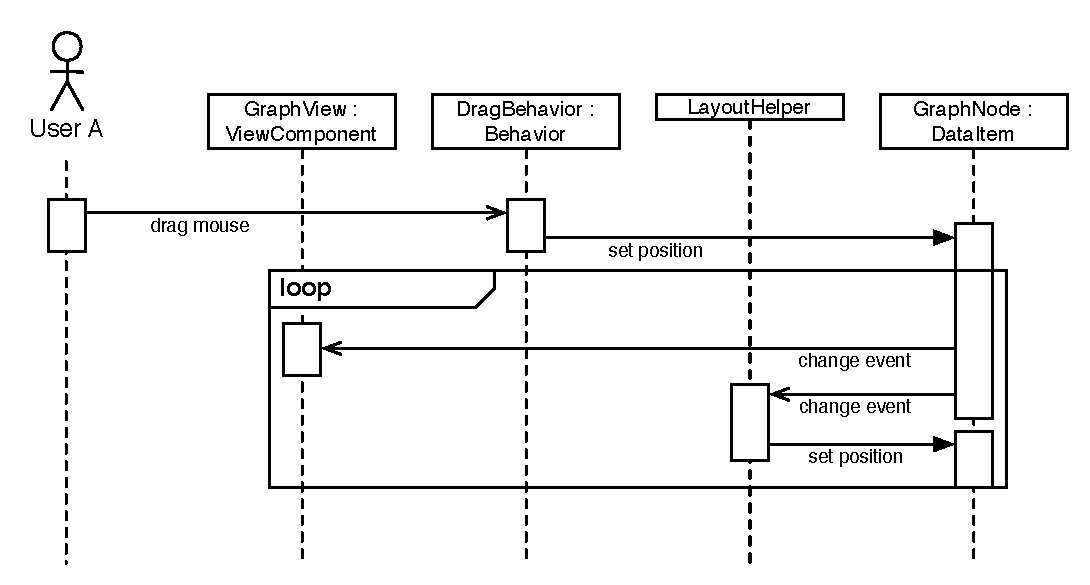
\includegraphics[width=0.7\textwidth]{cycle_seq.pdf}
\caption{An example of an infinite loop in the event system.}
\label{fig:eventcycle}
\end{center}
\end{figure}

When using an event-based system it is possible to create infinite execution loops. An example is shown in figure \ref{fig:eventcycle}. A common solution to that problem is to keep track of the object that initiated an event and omit event handlers of that object while propagating the event. \cite{Sommers_2009}

\section{Event congestion}
As shown in figure \ref{fig:eventcycle} some changes to data objects are triggered by native browser events, such as \texttt{mousemove}. Their frequency is determined by the sample rate of the input device (e.g. mouse or trackpad) and may be as high as 60 signals per second. This is a favorable effect, as it enables a lag-free user interface. However, as the event-driven architecture is designed to propagate change events not only within the client application but also to the server, this high event rate may lead to a congestion of the network connection. 
A solution to this problem is to throttle the network requests based on a fixed time interval. With this technique, temporary states in which the client has not yet completed his action, e.g. not released the mouse while still dragging, are also propagated to the server. Addressing this issue, there is another approach that only sends requests after there have been no events for a fixed time span. This mechanism, which is called \textit{debouncing}, is used for the client's synchronization with the server. \cite{Walsh_2012}


\chapter{Evaluation}

This section explains how the proposed architecture of Project Zoom enables the use cases and meets the requirements that were previously established.

\begin{figure}
\begin{center}
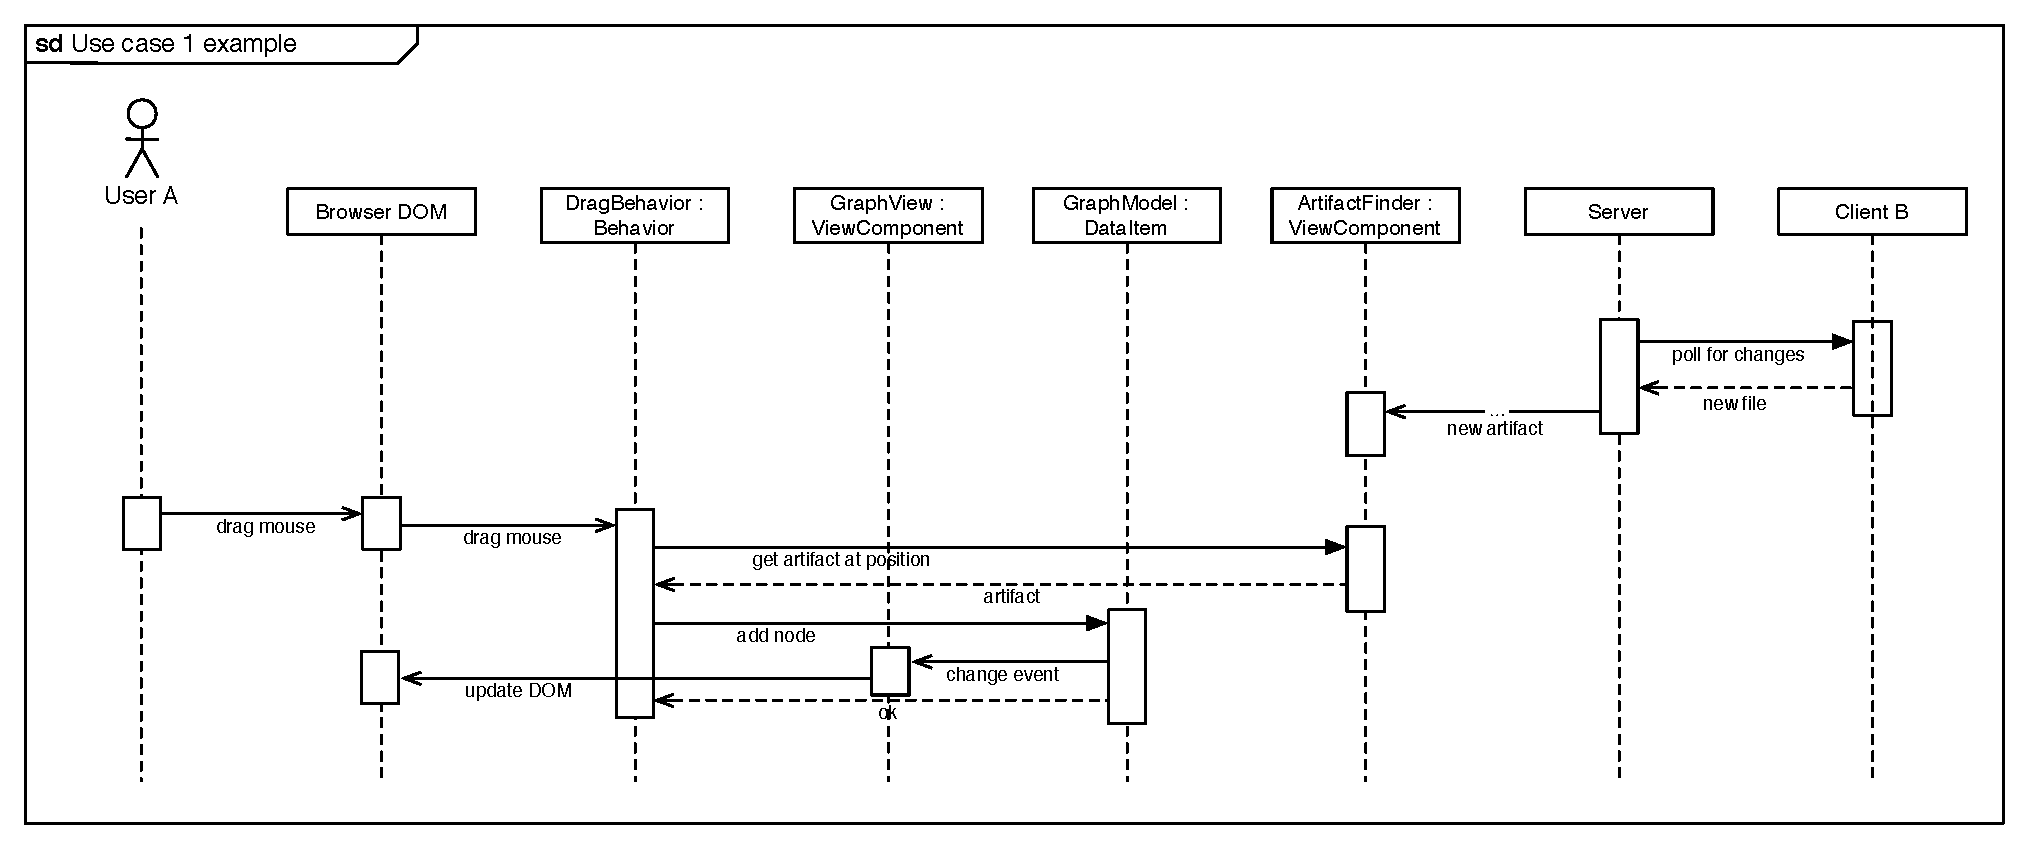
\includegraphics[width=\textwidth]{uc1_seq.pdf}
\caption{Sequence diagram for use case 1.}
\label{fig:evaluc1}
\end{center}
\end{figure}

\paragraph{\ref{uc:organize}} \textit{Student teams document their projects by organizing the digital documents they created, in a visual manner.}\\
Figure \ref{fig:evaluc1} shows how files are pulled from a storage provider by the server\footnote{Werkmeister covers how the data is pulled from different kinds of storage providers, e.g. \textsc{Box} and \textsc{Filemaker}. \cite{Werkmeister_2013}} and sent to the client. Because of the implemented dragging behavior, a user is able to add these documents as a node to the visual graph. Using context-sensitive actions these nodes may be connected to others or annotated in different ways \cite{Herold_2013}. 

\begin{figure}
\begin{center}
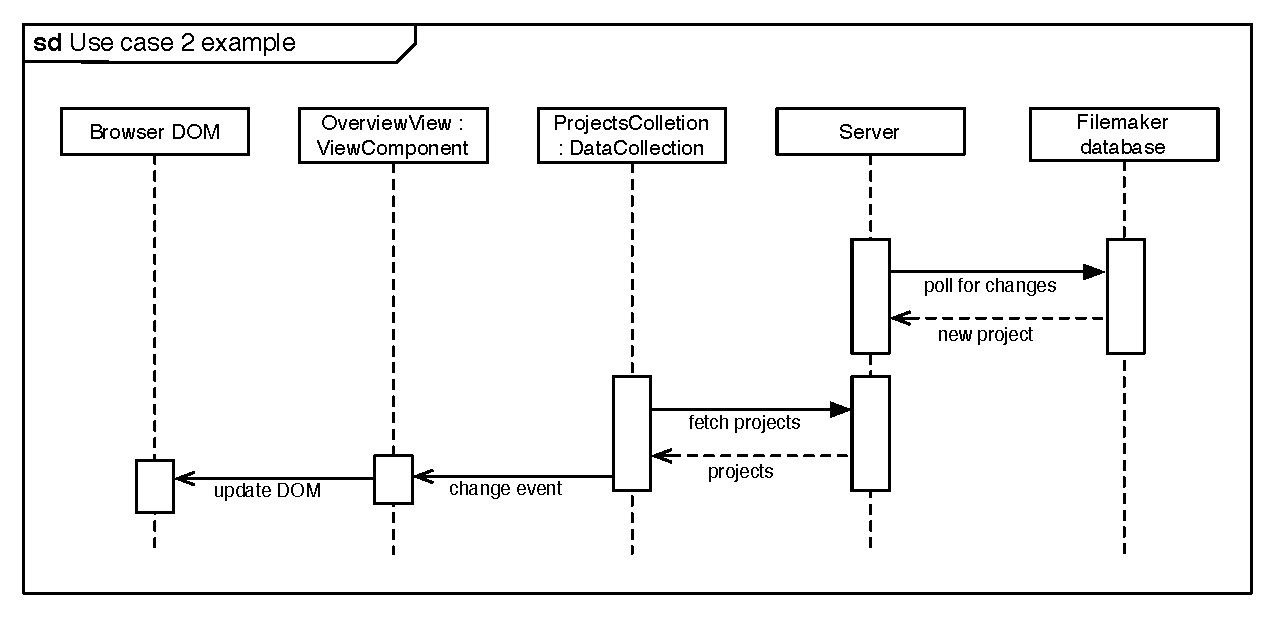
\includegraphics[width=0.7\textwidth]{uc2_seq.pdf}
\caption{Sequence diagram for use case 2.}
\label{fig:evaluc2}
\end{center}
\end{figure}

\paragraph{\ref{uc:display}} \textit{D-School staff members get an overview of all projects. This overview enables access to the projects' classifications, related people and documentations.}\\
The D-School uses a \textsc{Filemaker}\footnote{Filemaker, \url{http://www.filemaker.com/}, accessed 06/16/13} database to store projects. The server polls that database. The client can then access them through a REST interface and display them in a user interface. This interaction is outlined in figure \ref{fig:evaluc2}.

\paragraph{\ref{uc:fromhome}} \textit{The students add additional documents from their computers at home.}\\
Project Zoom is designed to use a web-based client-server architecture. The server software is capable of handling requests from clients over a network connection. If the software is deployed on a public server, the application will be reachable from any internet-connected computer. Use case \ref{uc:fromhome} requires the users to have an installation of an HTML5-capable browser to access the application. Such web browsers are very popular and likely to be already preinstalled on the user's computer.

\paragraph{\ref{uc:versions}} \textit{Students, teachers and D-School staff members can retrieve versions of the knowledge graph at different points in time.}\\
When a graph in Project Zoom has been edited, it is automatically stored shortly afterwards in the server's database. Every version of a particular graph is kept in the database for later retrieval \cite{Bocklisch_2013}. The server's REST interface includes a method for retrieving a specific version of a graph (cf. Appendix \ref{appendix:REST}).

\paragraph{\ref{uc:storageproviders}} \textit{Students can access the documents they saved using different commonly-used storage pro\-vi\-ders, e.g. Box.}\\
D-School students store the files they create in their projects using cloud storage providers, e.g. \textsc{Box}. The server includes a connector to the \textsc{Box} API. The extensible architecture of the server also allows to integrate with other services \cite{Werkmeister_2013}. Because of the event-driven architecture of the client, added files are displayed in the user interface after a very short time (cf. figure \ref{fig:evaluc1}).

\begin{figure}
\begin{center}
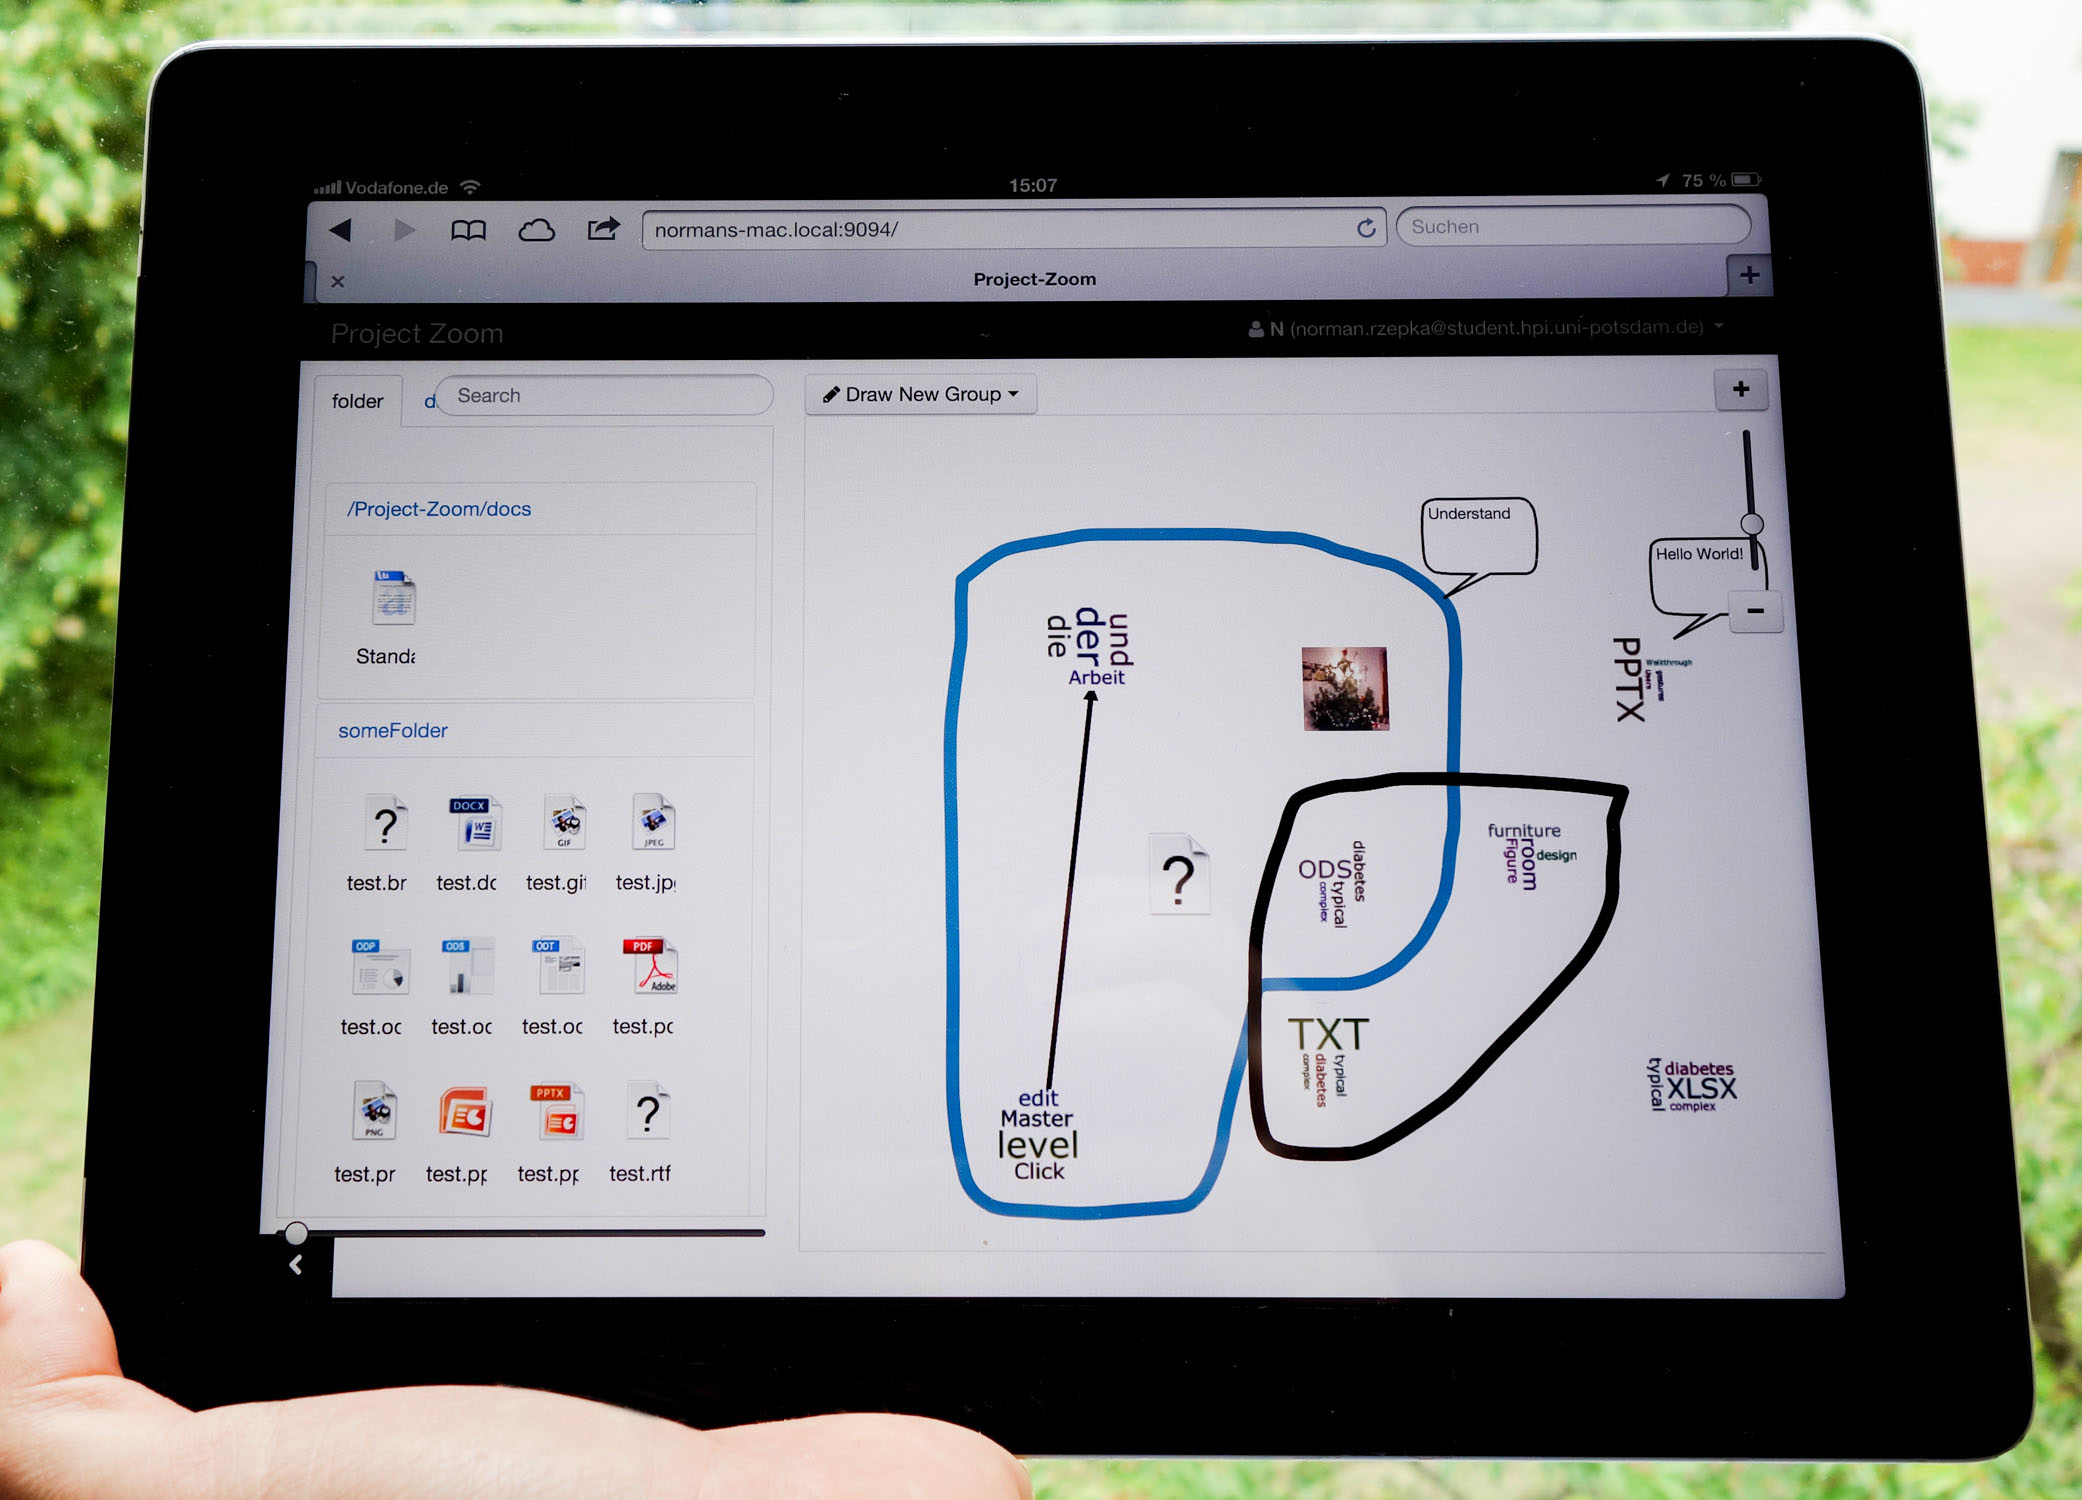
\includegraphics[width=0.5\textwidth]{ipad.jpg}
\caption{Photo of Project Zoom running on an Apple iPad (3rd generation).}
\label{fig:evaluc6}
\end{center}
\end{figure}

\paragraph{\ref{uc:multiplatform}} \textit{The Head of D-School and Program Managers show an overview of a filterable set of pro\-jects to potential industrial partners. Optional:  A mobile tablet device is used for the presentation.}\\
The D-School runs a variety of students projects. Using the \textsc{Filemaker} database, Project Zoom is able to display them in the user interface. Users are able to select a filter, which only shows the matching items \cite{Dieckhoff_2013}. Since the client of Project Zoom is implemented using HTML5 technologies, it also runs on popular mobile tablet devices, as demonstrated in figure \ref{fig:evaluc6}.

\paragraph{\ref{req:multiplatform}} \textit{The system's interface has to support multiple platforms, including the popular desktop operating systems and modern tablet devices.}\\
The requirement \textbf{\ref{req:multiplatform}} has already been covered by \ref{uc:multiplatform}.

\paragraph{\ref{req:fromhome}} \textit{The system's interface has to be accessible from outside the D-School.}\\
The requirement \textbf{\ref{req:fromhome}} has already been covered by \ref{uc:fromhome}.

\paragraph{\ref{req:concurrency}} \textit{The system has to support concurrent users accessing and modifying contents. \textit{Simplifying assumption}: A resource (e.g. a project's graph) can only be modified by one user at the same time. However, multiple users may edit different resources and any user can read any resource.}\\
Due to the nature of a web application, multiple clients can connect to a server. Thus, multiple users can access the same application concurrently. The system does not impose restrictions on concurrent read access through the client's user interface for any resource. An Operational Transformation algorithm is applied to provide a real-time collaboration experience and ensure eventual consistency. Because of the very basic handling of consistency conflicts, concurrent editing of the same resource (e.g. a graph) is not supported in the current implementation and subject to future work.

\paragraph{\ref{req:storageprovider}} \textit{The system connects to different data sources, e.g. Box and Filemaker, and makes the stored data available through its GUI.}\\
The requirement \textbf{\ref{req:storageprovider}} has already been covered by \ref{uc:storageproviders}.
